\label{sec:c}
The controller

\subsection{Relevant Files}
\begin{tabular}{|l|p{120mm}|}
\hline \textbf{File}  & \textbf{Description} \\ 
\hline controller.sv & Contains instruction decode logic to control datapath flow. Also includes micro operation state machine, exception handler, and program status registers.\\ 
\hline micropsfsm.sv & Mealy finite state machine that decodes complex instructions into sequences of simpler instructions. The instruction output by this module is used in the remaining controller decode logic.\\ 
\hline shift\_control.sv & Selects shift types, decodes shift amount, and determines shifter carry out from datapath barrel shifter. \\ 
\hline alu\_decoder.sv & Generates control signals for the ALU operation, inputs, and flags.\\
\hline memory\_mask.sv & Generates memory mask for storing different subsets of complete data words. \\
\hline conditional.sv & Checks conditional execution and kills writeback signals if an instruction should not be executed. Also generates the resultant flags of an instruction.\\
\hline exception\_handler.sv & A Mealy state machine that choreographs stalls, flushes, and branching when interrupts or exceptions are detected.\\
\hline cpsr.sv & Contains current and saved program status registers. Handles flag updates and verifies mode changes. \\
\hline 
\end{tabular} 


\subsection{Decode}
The controller Decode stage receives an instruction from the micro op FSM and generates datapath control signals.
Many control signals are needed for the execute, memory, and writeback stages. 
These are pipelined to follow the corresponding instruction, including any flushes or stalls.

\subsection{CPSR and Flags}
After a CPSR update the new flags and mode bits are forwarded to the next instruction before propagating to the writeback stage. 
This ensures correct operation of conditional and privileged instructions.

\subsection{MicroOp State Machine}\label{sec:uop}


\begin{figure}[h!]
\centering
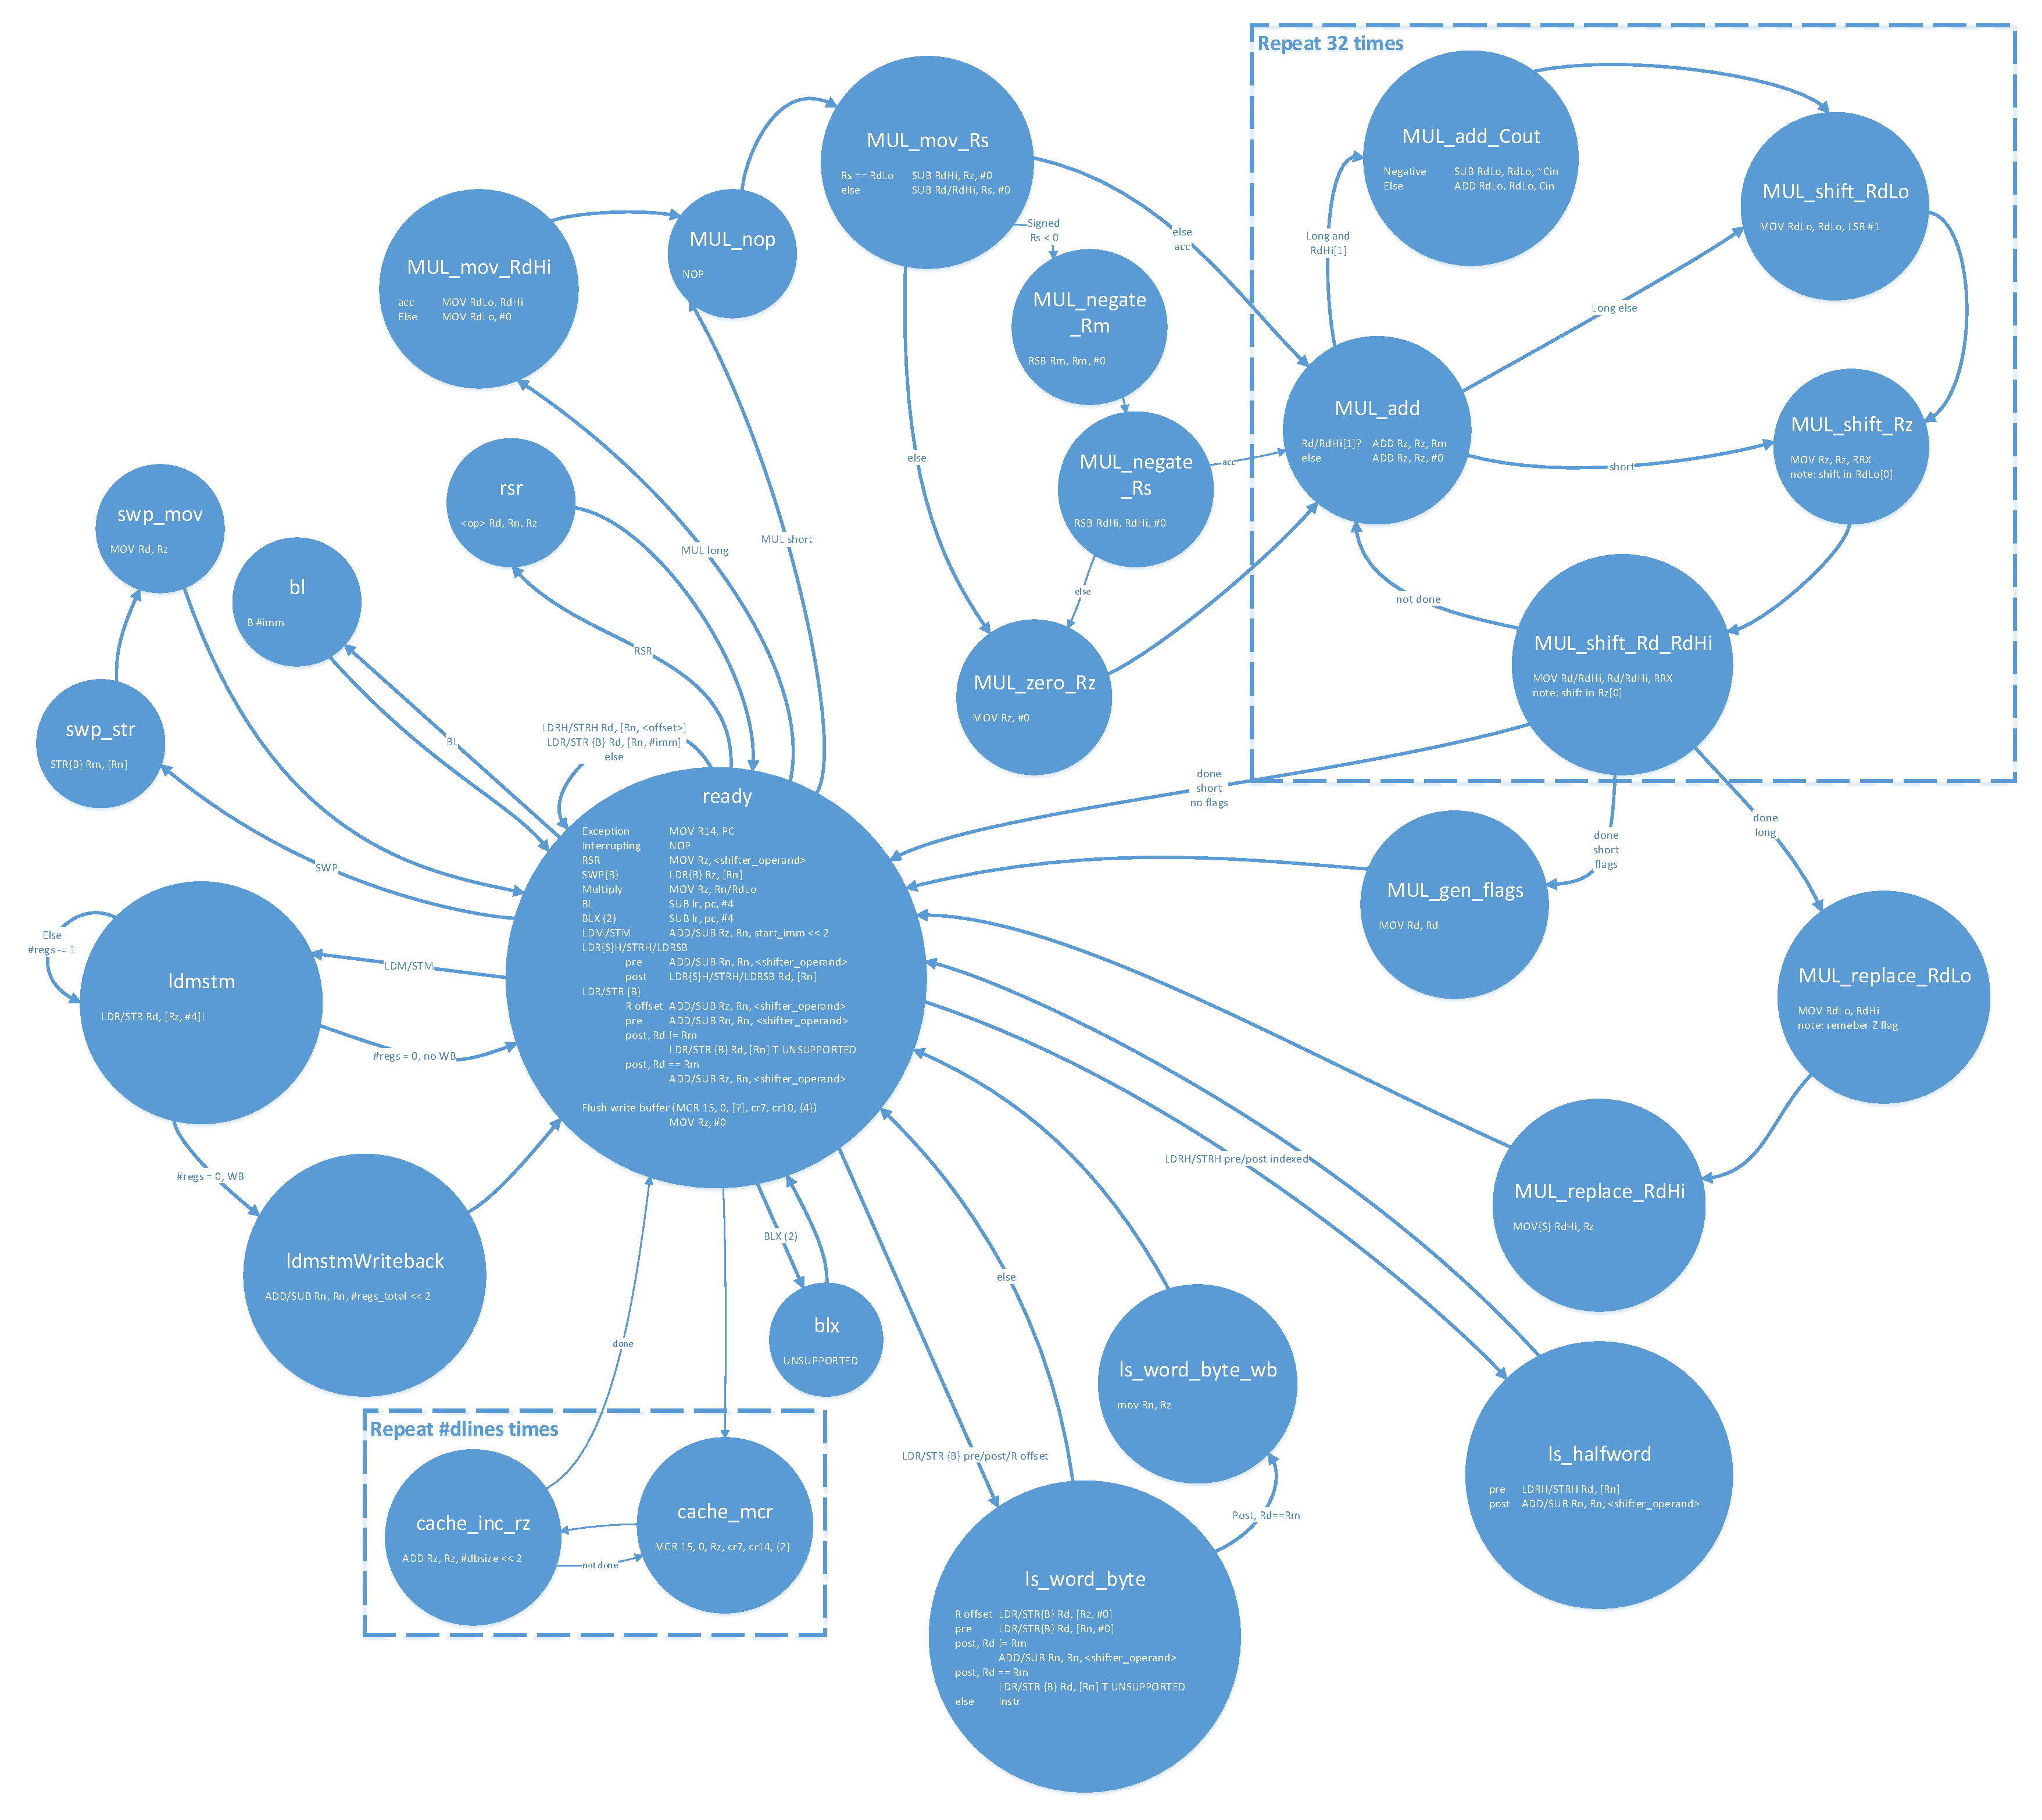
\includegraphics[width=\textwidth]{./diagrams/micropfsm_drawing.pdf}
\caption{State transition diagram for the micro op state machine. A high quality PDF is available as \texttt{documentation/diagrams/micropfsm\_drawing}}
\label{fig:uopdiagram}
\end{figure}

\subsection{Exception Issue State Machine}
